\chapter{Background}
\label{background}

In this chapter, we provide helpful background on geospatial data and software. We describe the standardized concepts and programming interfaces RAPID builds upon, as well as the inspiration and direction we've taken from related work.

\section{Introduction}
\label{background_intro}
RAPID's connected DSS make use of spatial data;\footnote{A note on terminology: some groups make a subtle distinction between ``spatial'' data and ``geospatial'' data. In those cases, spatial data describes data ``distributed in three-dimensional space,'' with ``measurable'' dimensions~\cite{Bhatta2011}. Given \textit{geography}'s definition, geospatial data is ``spatial data which is related to the Earth''~\cite{Bhatta2011}. In this project, spatial data is always located on Earth, so ``spatial'' and ``geospatial'' will be used interchangeably. As one supporting source, the United States Geological Survey considers ``the terms `spatial' and `geospatial' [to be] equivalent''
\cite{Bhatta2011}.} their eventual goal is to lay out and recommend pipeline routes through areas with as few hazards as possible~\cite{Dunning2013}. As such, this end-to-end system can be considered a spatial DSS (SDSS). SDSS are uniquely tasked with providing ``easy access to spatial data and decision models through the integration of spatial databases, analytical models, and visualization tools''~\cite{RedlandsSDSS}. RAPID is tasked with managing the spatial database and has to account for geographic information systems' (GIS) mathematical foundations.

This chapter describes \begin{enumerate*}[label=\itshape\alph*\upshape)]
\item basic GIS concepts,
\item structured and unstructured geospatial data formats,
\item spatial database management system usage, and
\item related standards
\end{enumerate*}. These have all played into RAPID's origins, design, and implementation.

\subsection{Open Geospatial Consortium}
The Open Geospatial Consortium (OGC) is an international consortium---with several hundred industry, government, and academic participants---whose goal is to establish standard formats and interfaces for geospatial data and applications~\cite{ogc}. Many organizations insist on using OGC-compliant products and services to promote robustness and interoperability, and they've created over thirty-five standards, which often include API specifications and markup languages~\cite{ogc,Dunning2013}. While not a top-to-bottom OGC-compliant system, RAPID utilizes and implements components of OGC Standards and is still useful for building on the same foundational concepts.

\section{GIS}
A GIS is a computer system (including hardware and software) for working with geographic data---that is, data associated with a location in space~\cite{Esriintro,gentle_intro}. Quite simply, GIS provide a means of viewing and managing this data. More importantly, GIS allow people to understand deep, complex information about geographic locations, their relative positions, and the objects and conditions that are located there~\cite{Esriintro,gentle_intro}.

Because many everyday and large-scale tasks and concerns are related to specific locations, so too are the computer applications that people use: from flight scheduling to car navigation, weather prediction, and social networking~\cite{Esriintro}. RAPID and its related applications, with their geospatial data, enable similar possibilities.

\paragraph{SDSS.}
The terms ``GIS'' and ``SDSS'' sometimes overlap ambiguously~\cite{Peterson}. GIS might only involve general-purpose geography and cartography, but SDSS have the specific goal of improving geospatial analysis and resource management~\cite{Peterson}. As such, SDSS \textit{use} a GIS or could be considered a \textit{type} of GIS~\cite{Peterson}.\footnote{The actual analyses are outside our work's scope.}

\subsection{Functionality}
GIS functionality can usually be placed in one of five categories~\cite{Esriintro}:

\begin{description}
  \item[Mapping object locations.] Descriptors can be assigned to points in space (take addresses, for example). In a technical sense, this is usually seen as associating string-like data---ideas or concepts (like place names)---with floating-point latitude and longitude. These are commonly called \textit{features} (central to any geospatial system)~\cite{Kottman2009}.
  \item[Mapping quantities.] Quantities can be mapped to certain points to relate locations with numeric data about them. This could be integers and floating point values, again, assigned to latitude and longitude. These are also considered features.
  \item[Mapping densities.] Not only can values be assigned to specific points on a map, densities can be generated and displayed, which show the distribution of objects or values over an area.
  \item[Determining relative positions of objects.] GIS can determine if spatial entities are located within or near each other. Additionally, they measure distances between objects and locations and determine whether or not they intersect.
  \item[Analyzing trends.] Many GIS look at trends in data. There's a lot of demand and opportunity for analysis in how locations and features change over time.
\end{description}

In summary, GIS capture, manage, analyze, and display geographically-referenced information; viewing and understanding the relevant patterns can be done with maps, graphs, and written reports~\cite{Esriintro}. RAPID, at a low level, acts as a foundation for that functionality.

\section{Data characteristics}
This section outlines more technical considerations for geospatial data, which is not always easily represented or stored in common formats. Although humans often notate points in space with numbers (and, occasionally, symbols) it's best to treat them as their own primitive data type in software for friendliness and robustness~\cite{gentle_intro}.

Because of this, geospatial data structures and file formats must be able to specify points in two or three dimensions: latitude, longitude, and elevation (if desired).\footnote{Conceptually, time can be viewed as an additional dimension---one of a feature's properties---so the data is geospatial-\textit{temporal}. RAPID includes a timestamp on its data and allows filtering based on that timestamp.} GIS and spatial database management systems often need to account for any arbitrary coordinate system~\cite{gentle_intro}.

Considering the above, two common file and data types have emerged in GIS: vector and raster. They are briefly described below. We preface this with a needed introduction to standardized geographic concepts from the OGC, including particulars on coordinate and projection system usage.

\subsection{Abstract Specification}
OGC's Abstract Specification describes and standardizes the essential components of geospatial data, including the central information model and glossary for all OGC Standards~\cite{AbstractSpecFaq}.

Any sizable geospatial software system is naturally governed by certain geographic and geometric properties and functions; the Abstract Specification is the OGC's formalization of those concepts, all of which are encompassed in the data types and formats in the upcoming sections~\cite{AbstractSpecFaq}. The idea of a geospatial \textit{feature} (described above), for instance, is an essential concept~\cite{Kottman2009,AbstractSpecFaq}.

\subsection{Simple Features Access}
One foundational OGC standard, Simple Features Access (ISO 19125) defines the official data storage and access model for geospatial features~\cite{SFA}. As with many other standards and GIS-focused designs, Simple Features Access builds directly on the Abstract Specification's established concepts~\cite{SFA,AbstractSpecFaq}. The SQL statements and spatial operators described later in this chapter are directly shaped by the Simple Features Access standard.

\paragraph{Projection.}
There are many different mathematical and geographic coordinate systems and projections---created and suited for different tasks---but they aren't necessarily compatible with each other~\cite{Kottman2009}. OGC standardizes unique Spatial Reference System Identifiers (SRIDs) in Simple Features Access to differentiate in-use coordinate systems~\cite{SFA}. To correctly identify, parse, and measure geometries, they must have a specific, known SRID~\cite{Kottman2009}.
  
In common with other GIS defaults, we specify RAPID to use SRID 4326, the standard World Geodetic System (WGS 84)~\cite{Nima2000,SFA}. WGS 84 utilizes the latitudes and longitudes most people know (from -90\textdegree~to 90\textdegree~and -180\textdegree~to 180\textdegree, respectively), and it's used in GPS~\cite{Nima2000}.\footnote{Data imported into RAPID using other SRIDs must (and can) be transformed to SRID 4326 before performing spatial queries. This process is briefly described in Chapter~\ref{design}.}

\subsection{Vector}
\label{sec:vector}
Vector files contain mathematical and geometric representations of spatial data, defining points and shapes in space. They are split into two components: geometries and attributes (or ``properties'').

\subsubsection{Geometries.}
Coordinate pairs are two values that represent a point in space in a coordinate system~\cite{gentle_intro}. Most commonly (and in RAPID), this is WGS 84, where one value is latitude and other is longitude; taken together, any point on Earth's surface can be represented.

In vector files, sequences (or ``series'') of these points can represent different geographic concepts, most often called ``geometries.'' There are Points, Lines, Linestrings, and Polygons (shown in Figure~\ref{fig:geoms})~\cite{gentle_intro}:

\begin{description}
  \item[Points.] Points include the necessary coordinates to designate one position in space. See Figure~\ref{fig:point}.
  \item[Lines.] Lines are drawn from one Point to another (and are represented by the ordered pair). See the Linestring in Figure~\ref{fig:linestring}, which is composed of three Lines.
  \item[Linestrings.] Linestrings are multiple connected Lines (and, thus, chained pairs of Points). These can represent objects or markers like road networks or pipelines. See Figure~\ref{fig:linestring}.
  \item[Polygons.] Polygons are Linestrings where the last Point is equal to the first---creating a closed shape. Political borders in the United States are a good example: the country is broken up into polygonal states, and states are broken up into polygonal counties, cities, and congressional districts. See Figure~\ref{fig:polygon}.
  \item[Polygons with holes.] Holes can be added to the interior of Polygons: the main, outer Polygon is represented by one Points series, and subsequent Point series represent internal gaps. See Figure~\ref{fig:polygonhole}.
\end{description}


\begin{figure}
    \centering

      \subfloat[Point]{\label{fig:point}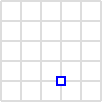
\includegraphics[width=0.2\textwidth]{figures/point.png}}
      \hfill
\subfloat[Linestring]{\label{fig:linestring}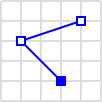
\includegraphics[width=0.2\textwidth]{figures/linestring.png}}
       \hfill
      \subfloat[Polygon]{\label{fig:polygon}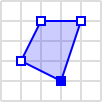
\includegraphics[width=0.2\textwidth]{figures/polygon.png}}
      \hfill
        \subfloat[Polygon with hole]{\label{fig:polygonhole}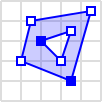
\includegraphics[width=0.2\textwidth]{figures/polygon_with_hole.png}}
    \caption{Standardized geometries from OGC's Abstract Specification}
    \label{fig:geoms}
    
\end{figure}

\subsubsection{Attributes}
Attributes are simply non-spatial data that's associated with the spatial data described above. An address (also mentioned above) is a great example: house numbers, streets, cities, states, and zip codes all associate an identifier with a point in space (or other geometric type)~\cite{gentle_intro}.

\subsection{Raster}
Raster data is simply grids of values. It's best to imagine a digital image: pixels in a matrix are each assigned red, green, and blue color values. When they're appropriately combined and visualized, a continuous dataset spreads over a region in two or three dimensions~\cite{gentle_intro}. Images, in fact, are a type of raster data often found in GIS (like satellite images). Atmospheric or ground sensors can also provide data sets that blanket an area~\cite{gentle_intro}.

Because raster data is continuous over a region, programs and users need to account for the \textit{density} of data---that is, the size of each grid cell, which is referred to as ``resolution''~\cite{gentle_intro}. Resolution is either spatial or spectral:

\begin{description}
  \item[Spatial.] Spatial resolution is how large a cell of the grid is and how it corresponds to a real geographic area~\cite{gentle_intro}. For example, a side of one cell could be four feet.
  \item[Spectral.] Spectral resolution is the number of color ``bands'' in raster images~\cite{gentle_intro}. In an ordinary image, red, green, and blue are these three bands---the spectral resolution~\cite{gentle_intro}. In some cases, images may also capture infrared or ultraviolet light and store more data in other color bands~\cite{gentle_intro}.
\end{description}

\textit{Georeferencing} makes raster data useful geographically: it associates the raster data with a location. For example, a GIS that displays a satellite image of California on top of an interactive state map can calculate where real geographic features are in the image~\cite{gentle_intro}.

With these four pieces of information (and some accompanying calculations), a raster file can be properly georeferenced and positioned in a coordinate system \cite{gentle_intro}:

\begin{itemize}
  \item Coordinates of the file's top-left pixel
  \item Width of a pixel
  \item Height of a pixel
  \item Rotation of the grid
\end{itemize}

\section{Data storage}
\label{storage}
This section overviews several storage considerations for GIS data.

\subsection{Database management systems}
Because of the unique data considerations described earlier, databases that manage geospatial data need to pay special attention to the methods of doing so. Spatial database management systems (spatial DBMS) provide ways of storing and querying geospatial data~\cite{Boundless}. This includes syntax for adding vector and raster data types~\cite{Boundless}.

\paragraph{Example.}
\label{background_wkt}
Inserting geometries (vector data) into a spatial DBMS can look like the following. We use a SQL statement to add geometries to a PostGIS table (RAPID's underlying database):

\begin{Verbatim}[samepage=true,baselinestretch=1,numbers=left,xleftmargin=12mm]
CREATE TABLE geometries
 (name varchar, geom geometry);

INSERT INTO geometries VALUES
  (`Point',
   `POINT(0 0)'),
  (`Linestring',
   `LINESTRING(0 0, 1 1, 2 1, 2 2)'),
  (`Polygon',
   `POLYGON((0 0, 1 0, 1 1, 0 1, 0 0))'),
  (`PolygonWithHole',
   `POLYGON((0 0, 10 0, 10 10, 0 10, 0 0),
   (1 1, 1 2, 2 2, 2 1, 1 1))'));

SELECT name, ST_AsText(geom)
FROM geometries;
\end{Verbatim}

These SQL statements demonstrate the creation of four geometries in a geospatial database: a single Point, a Linestring, Polygons, and Polygons with holes. Note that the generic \texttt{geometry} data type, shown in the \texttt{geometries} table above, is also standardized in Simple Features Access, which can store any of the more specific geospatial types~\cite{Boundless,SFA}.

In terms of notation, the space-separated numbers are a coordinate pair. Commas separate the points, creating ordered series. This particular syntax is Well-Known Text (WKT), an OGC Standard for defining Abstract Specification geometries~\cite{ogc}. Those five geometric data types in PostGIS---\texttt{POINT}, \texttt{LINE}, \texttt{LINESTRING}, and \texttt{POLYGON}---correspond to the types described above in Section~\ref{sec:vector}.

\subsubsection{Querying}
Simple Feature Access, introduced above, defines several required methods for comparing and relating Geometries, summarized below~\cite{SFA}. Figures~\ref{fig:touches} through~\ref{fig:within} visualize four of these boolean relational operators.

\begin{figure}
    \centering

    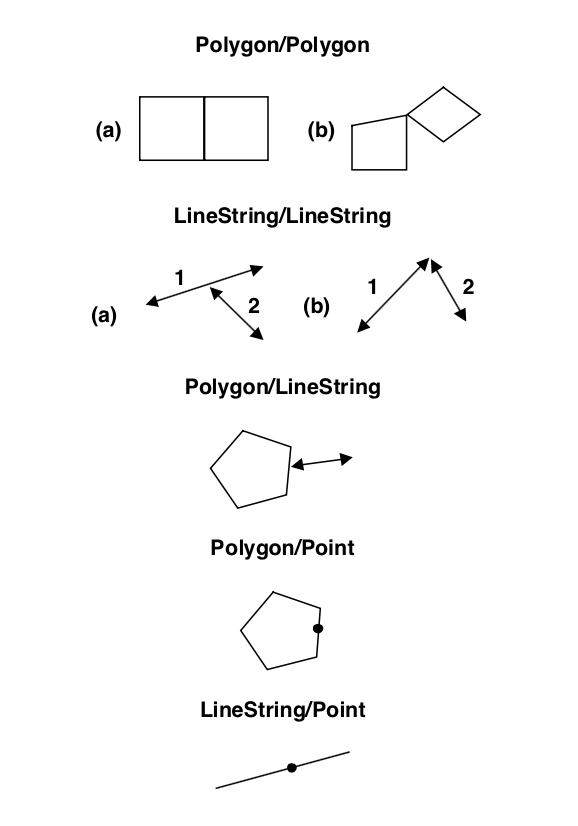
\includegraphics[width=0.45\textwidth]{figures/touches.png}
    
    \caption{Geometries exemplifying the `Touch' relationship}
    \label{fig:touches}
    
\end{figure}

\begin{figure}
    \centering

    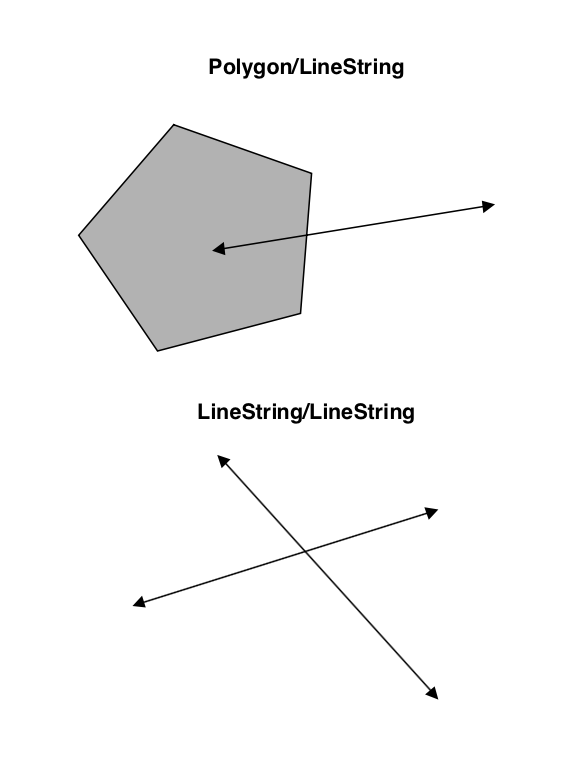
\includegraphics[width=0.4\textwidth]{figures/crosses.png}
    
    \caption{Geometries exemplifying the `Intersects' relationship}
    \label{fig:intersects}
    
\end{figure}

\begin{figure}
    \centering

    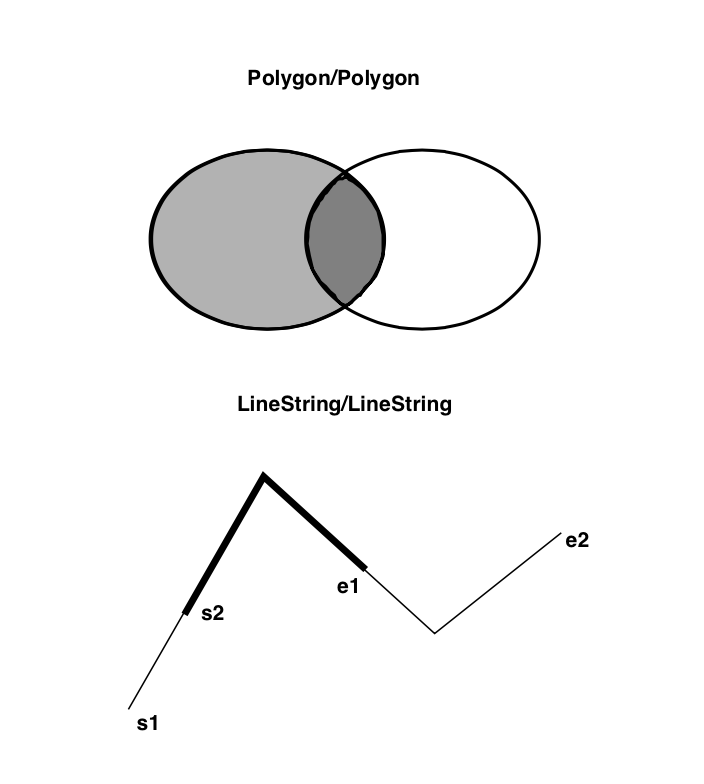
\includegraphics[width=0.5\textwidth]{figures/overlap.png}
    
    \caption{Geometries exemplifying the `Overlap' relationship}
    \label{fig:overlap}
    
\end{figure}

\begin{figure}
    \centering

    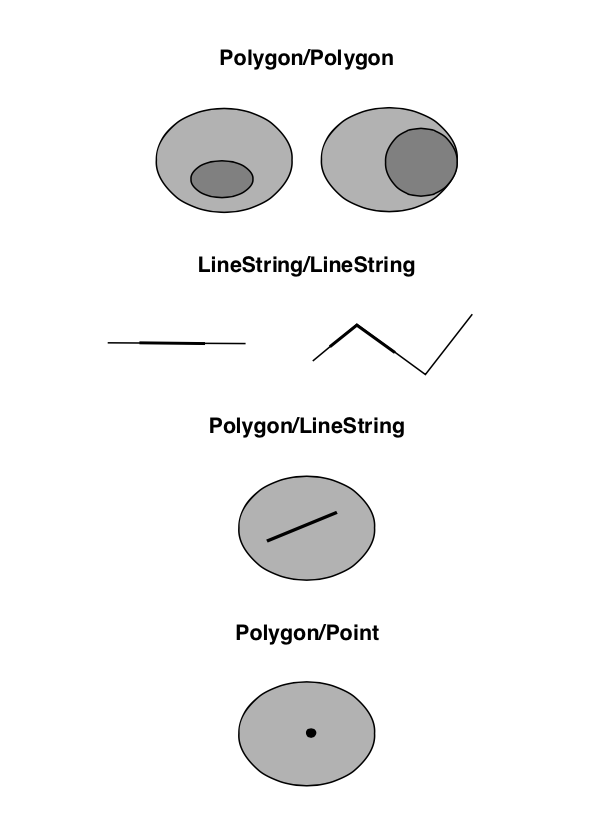
\includegraphics[width=0.45\textwidth]{figures/within.png}
    
    \caption{Geometries exemplifying the `Within' relationship}
    \label{fig:within}
    
\end{figure}

\begin{description}
  \item[Equals.] Tests for equality of two Geometries.
  \item[Intersects.] Tests whether the interiors of Geometries intersect.
  \item[Disjoint.] The opposite of intersection.
  \item[Cross.] Tests if the intersection of two Geometries is in one dimension fewer than the source Geometries.
  \item[Overlap.] Determines if the intersection of two Geometries is different from both the source Geometries but of the same dimension.
  \item[Touch.] Tests whether Geometries have their boundaries touching (without intersected interiors).
  \item[Within and Contains.] Test if a Geometry is fully inside of another.
  \item[Distance.] Calculates the shortest distance between two Geometries.
  \item[DWithin.] Tests whether Geometries are within a specified distance of each other.
\end{description}

It's easy to see where and why these come in handy. As a simple example, imagine that a mobile device stores its geographic location---a Point---and is trying to determine the city it's currently in. If a DBMS stores borders (Polygons) for cities, a query can be performed that asks if the Point is within cities' borders~\cite{Boundless}.

The queries below show some similar ideas that are unique to geospatial data: the first selects the neighborhood(s) that the Broad Street subway station is located in, and the second selects points of interest within 1609 meters of any road.

\begin{Verbatim}[samepage=true,baselinestretch=1,numbers=left,xleftmargin=12mm]
SELECT nyc_subways.name, nyc_neighborhoods.name
FROM nyc_neighborhoods
JOIN nyc_subways
ON ST_Contains(nyc_neighborhoods.geom, nyc_subways.geom)
WHERE subways.name = `Broad St';
\end{Verbatim}

\begin{Verbatim}[samepage=true,baselinestretch=1,numbers=left,xleftmargin=12mm]
SELECT roads.roadname, pois.poiname
FROM roads
JOIN pois 
ON ST_DWithin(roads.geom, pois.geom, 1609);
\end{Verbatim}

This type of analysis can be done application-side (as opposed to in the database) but DBMS technologies have advanced enough that this type of data can be stored and queried very efficiently, with user-friendly queries like above~\cite{Boundless}.

\subsection{Files}
\label{background_formats}
As can generally be the case with file formats and proprietary or fragmented software, geographic file formats are numerous and varied. Several come from cartographic- and surveillance-focused government agencies, like the United States Geological Survey and the National Geospatial-Intelligence Agency~\cite{UsgsStandards}. Other GIS vendors may have their own file considerations and requirements~\cite{slashgeo,Environ1998,GeoJSON}.

\subsubsection{Esri Shapefiles}
A go-to file format for vectors is Esri's shapefile, which includes the two vector components described above: attributes and point data~\cite{Environ1998}. Shapefiles are a (mostly) open and standard format managed and developed by Esri for use within the GIS space (and particularly their popular software, ArcGIS)~\cite{Environ1998}. Although this isn't an OGC Standard, it's become a ubiquitous vector format for GIS.\footnote{Interestingly, Shapefiles have begun to show their age (they originated in the early 1990s), and there were calls for a more modern, robust shapefile format from the OGC, which resulted in GeoPackage, a modern vector format based on SQLite. Shapefile's ubiquity and history keeps it in widespread use, however ~\cite{slashgeo,GeoPackage}.}

Despite its singular name, a ``Shapefile'' is actually a set of several different file types~\cite{Environ1998}:

\begin{description}
  \item[\tt{.shp}] These files contain actual shape geometries.
  \item[\tt{.dbf}] These files store the non-spatial attributes that are associated with the geometries in the shapes file.
  \item[\tt{.shx}] These are index files that store metadata about entries' locations in a file and allow for seeking forward and backward between features.
\end{description}

\subsubsection{GeoJSON}
GeoJSON is another common vector file format, although it's not standardized by OGC. It stores data in a nicely-readable format---a superset of JSON (JavaScript Object Notation). Take this example of a geospatial feature in GeoJSON:

\begin{Verbatim}[samepage=true,baselinestretch=1,numbers=left,xleftmargin=12mm]
{ "type": "Feature",
    "bbox": [-180.0, -90.0, 180.0, 90.0],
    "geometry": {
      "type": "Polygon",
      "coordinates": [[[-180.0, 10.0], [20.0, 90.0],
                       [180.0, -5.0], [-30.0, -90.0]]]
    }
}
\end{Verbatim}

It should be apparent that this syntax corresponds closely to the Abstract Specification we've been discussing, with standardized geometry types notated by lists of Points (latitudes and longitudes in this case). Arbitrary, situation-specific properties can be appended in the same fashion as the key-value pairs above.

\paragraph{Bounding box.}
The \textit{bbox} attribute is a bounding box, which serves as an \textit{approximate} area---bounding, rectangular dimensions---for a geospatial feature~\cite{Boundless}. Although actual feature coordinates may describe a more intricate border, a rougher bounding box is less complex and more efficient to compute spatial queries for---sometimes a good-enough replacement for the slower (but precise) queries. In some cases, it's reasonable to check spatial queries on bounding boxes and, depending on the results, later check the true geometry for additional accuracy~\cite{Boundless}. A bounding box is not unique to GeoJSON and is commonly found in geospatial data specifications and APIs~\cite{Boundless}. 

See Figure~\ref{fig:bbox} for examples, which nicely shows the difference between querying bounding boxes and querying true geometries. Studying the bounding boxes, we'd quickly learn that \begin{enumerate*}[label=\itshape\alph*\upshape)]
\item each of the lines \textit{might} intersect with the Polygon but
\item the lines surely \textit{don't} intersect with each other
\end{enumerate*}. Examining the true shapes takes longer but reveals that \textit{none} of the geometries intersect.

\begin{figure}
    \centering
    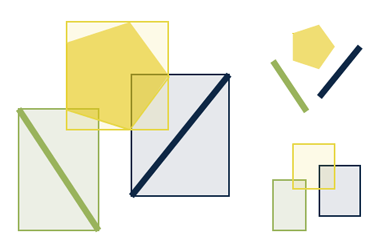
\includegraphics[width=0.5\textwidth]{figures/bbox.png}
    \caption{Bounding boxes shown for three example geometries.}
    \label{fig:bbox}
\end{figure}

\subsubsection{Related formats}
There are dozens of other geospatial file formats with certain specializations, degrees of standardization, and application-specific features, but Shapefiles and GeoJSON are nicely representative of their general capabilities and stylistic differences (and are RAPID's initially-support formats).